\documentclass{article}[11pt]
\textheight 8.5in
\usepackage{graphicx}
\usepackage{float}%for forcing position of figs
\usepackage{hyperref}


\begin{document}
\begin{center}
Siddharthan Rajasekaran\\
Week of 25/6/2012 - 1/7/2012
\end{center}
\section{Summary of Discussions}

Learning from demonstration is the process of a teacher demonstrating a task by means of teleoperating the robot with joystick or performing the task themselves and recording it and thus making robots learn from these examples. In this report we are trying to answer questions like What is LfD, whom , how and when to learn, what are the different ways we can record demonstrations, what are different ways we can follow these demonstrations, when does robot learning come into picture, etc. We also put forward some of the ideas in which we can improve existing algorithms.

\section{Papers Read}
In \cite{hbr}, the active part of Learning from Demonstrations (LfD) is covered. Wherein, the human is in the loop during the learning process of the robot. This is also referred to as active teaching. In active teaching the robot can ask for help during execution of demonstrations in real time when it does not know how to solve the task. This is mainly aimed at how traditional LfD can be augmented with such active teaching techniques to bring out better performance. It focuses on when and what question should be asked to get maximum information from teacher. 
In the survey \cite{argall2009survey} on LfD, they give a rather broader discussion on traditional LfD itself which includes learning from recorded demonstrations. 

A typical recording of a demonstration has a sequence of states and actions. Before these recordings can be executed on a real robot, we need to solve for several mappings. The first of the several mappings that has to be solved for is the recording mapping $g_R$ and embodiment mapping $g_E$. The former is the mapping from the states and actions experienced by the teacher to the ones that are recorded. Embodiment mapping is the mapping between the states and actions that are recorded to the the states and actions that are experienced by the robot while repeating the task. LfD can be categorized based on $g_R$ and $g_E$ which is shown in figure.\ref{fig:class}. 

\begin{figure}[H]
  \begin{center}
    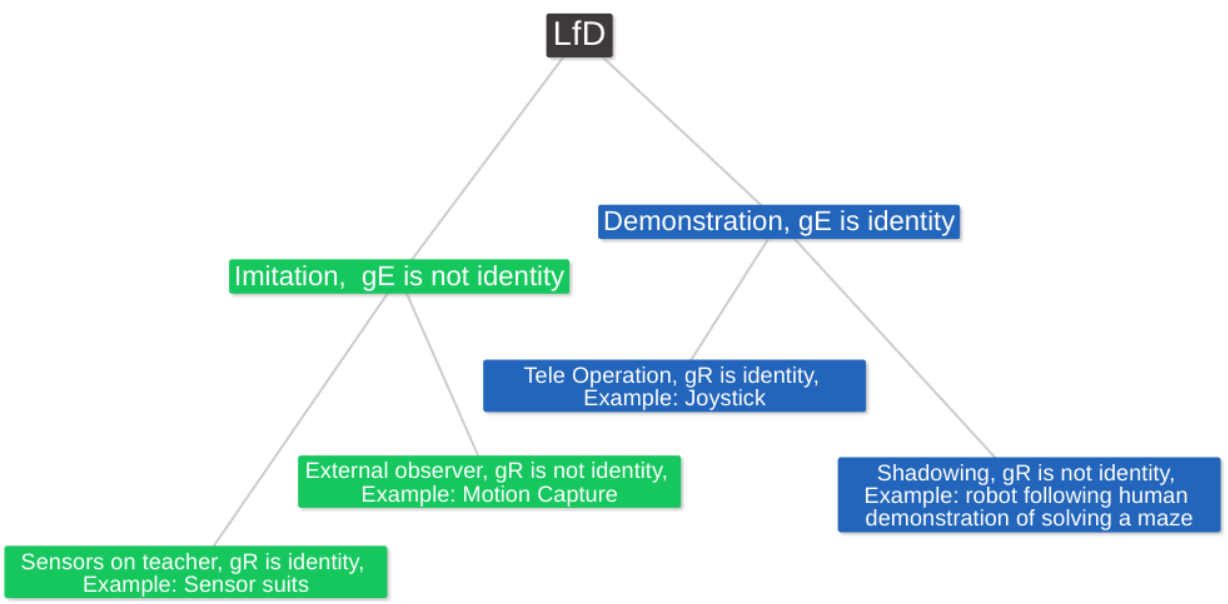
\includegraphics[width=1\linewidth]{images/classification}
    \caption{Classification of work in LfD based on the method of recording demonstrations and executing them.}
    \label{fig:class}
  \end{center}
\end{figure}


\subsection{Demonstration: $g_E = $ Identity}
	Here, the mapping between the recorded demonstration and the states and actions experienced by the robot during execution is identical. This subclass (demonstration) can be further divided based on whether the recording mapping is identity or not. 

\subsubsection{Teleoperation: $g_E = I, g_R = I$}
These are demonstrations in which the teacher performs the task on robot but by controlling remotely. Since the demonstration is done on the robot, it is easy to record the states and actions experienced by the robot using sensors attached to it. Hence these recordings have $g_E = I$ since during execution the robot need not apply any transformation to the available recording. Also the experience of the teacher comes from the robot since the teacher performs the task on the robot $\Rightarrow g_R = I$. Examples: using joystick to teleoperate \cite{invheli}, kinesthetic teaching \cite{fbm} (where the teacher moves passive joints of the robot) or through speech \cite{speech}. 

\subsubsection{Shadowing: $g_E = I, g_R \neq I$}
Here, the teacher performs the task, while the robot records the demonstration using its own sensor. The learner records the states and actions of it's own execution which has a non identity mapping to what the teacher experienced. Hence ($g_R \neq I$ and $g_e = I$). Examples include navigation tasks where a human teaches another robot by solving a maze. The learner records its experience since it is trying to figure out what to do while navigating autonomously \cite{shad}.

\subsection{Imitation}
 Here, the teacher performs the tasks by him/herself. Later, the recording of the demonstration is executed on the robot with the idea of imitating the teacher. Hence the embodiment mapping $g_E \neq I$. For example, while executing a manipulation task, a human demonstrator may move each joint differently from how a robot with redundant manipulator should move to achieve the same task in workspace. $g_E$ might be solving the inverse kinematics while minimizing some cost function per se.
 
\subsubsection{Sensors on teacher}
If the sensors are on the teacher while demonstrating, evidently the recording mapping $g_R = I$. Some examples include recording walking patterns by wearing sensor suits, recording drumming patters similarly. 
These methods alleviate finding the mapping $g_R$ while having to deal with the overhead of using such sensor suits in controlled environments. 

\subsubsection{External sensors}
In a similar setting of imitation one can also observe what the teacher is doing from outside. For example, the robot observes the teacher using its own sensor to record demonstration or the use of motion capture system. Though one has to deal with finding $g_R$, these methods are more general and we do not have to deal with the overhead of wearing sensor suits as in the previous case. 


\subsection{Findind a policy}

Once we have recorded demonstrations, we must find a policy on the robot which will effectively complete the same task. This is the part where ``learning" is  done. If we do not actually learn a ``common sense" out of these demonstration on what actually completing the task means, then we would simply be using the recording as a look up table from states to actions. Learning actually meets our objective by generalizing well. 

The aim here is to derive a mapping function from observed states to actions. There are several work which addresses issues like when to do function approximation (before or during execution), what to use in case of continuous or discrete state and action settings, should the algorithm update online and should we keep the entire dataset of demonstration throughout or some minimilistic representation.

These methods heavily are drawn from traditional machine learning (for learning actions) and reinforcement learning(for learning system dynamics/actions) approaches. In discrete setting, classifiers can be used to learn three types of action 1) Motion control 2) Action primitives 3) Complex behavior. We will look at some of the examples and what algorithms are used (we won't be going into the details of the algorithm) so we can get an idea of what is out there. 

Learning low level actions (motion control) has been demonstrated by controlling a car using Gaussian Mixture Models \cite{car}, controlling a airplane using decision trees. HMMs have also been used to learn a rather complex task (flipping eggs using manipulator) which is an example of using action primitives. There are examples of extracting the action primitives from a demonstration using hierarchical neural nets (different neural nets used for different purposes instead of doing end-to-end learning). Neural nets have also been used to perform complex actions like autonomous driving and using manipulator to solve peg in hole task. Learning complex actions include lazy learning wherein an unlabeled observation is labeled simply using kNN is also an example of learning in this context. In addition to this, Gaussian Linear Regression and Gaussian Process regression have been used in this area too.

Another thing to be learned other than the state action mapping itself is the system model. Often, in learning literature, it is common to model the world where we have to make control decisions as a Markov Decision Process (reviewed last week 2/18 - 2/25) where the dynamics of the system is given by the transition probabilities $T(s'|s,a)$, which gives a distribution over possible resultant states $s'$ given that we take action $a$ from state $s$. The optimal policy that maximizes cumulative reward in this setting is given by $\arg \max_\pi \int_t \gamma^tr(s_t|\pi)$. Reinforcement learning can be done either model-based or model-free. In the interest of learning the system dynamics one might want to use model based approaches. But in LfD context there is significant work in combining model free RL to actually perform the task better than the original demonstration. We are able to perform better only because most of the demonstration from teachers are often a feasible solution and not the optimal one. 

Some methods use hand-engineered reward functions while others use demonstrations to learn the reward function itself. 

\subsubsection{Hand-engineered reward function}
Often in reinforcement learning, it is hard to choose a reward function whose maximum occurs at our required behavior \cite{fault}. One solution to this is to have reward functions that are exceptionally sparse. That is, they have some high value at goal state and zero or the same negative values at all other states. This makes it very hard for the agent to explore a plethora of policies to hit the goal by chance and hence start improving on the policy. Often, most policies do not lead to the goal state and hence all policies would look similar for the agent (equally bad) which makes us rely on random exploration rather than hitting the goal with some directed search. For example, take the task in which a robotic manipulator has to tie a knot using a rope. Let the reward by $+100$ when the knot is successfully tied, zero otherwise. It is easy to imagine that it is very unlikely to hit the goal state even once merely by random exploration. Hence demonstrations by teachers can bias the search towards regions where we can be more optimistic to find the optimal policy \cite{brys2015reinforcement}. in many cases it is also dangerous to explore using random policies.  


\subsubsection{Learning the reward function}
Here, we learn the reward function given the demonstration. This is the typical case of Inverse Reinforcement Learning \cite{irl}. There are also works in which traditional RL algorithm is modified to ask the user to label reward to states experienced by the robot. 

\subsubsection{Acting in undemonstrated states}   
From the above methods, we can see a wide range of function approximation used to tackle the problem of visiting states that are not in the recorded demonstration. However, it is also good to define a default stabilizing behavior for our learning algorithms to generalize more safely. These stabilizing behaviors can be derived from optimal controllers. For example iterative LQR is used in case of continuous and Monte Carlo tree Search (MCTS) is used in case of discrete domains \cite{mcts} in order to train Neural Networks. The motivation to use learning in place of optimal control during execution is that it is often computationally more expensive to solve optimal control problem that to feed forward through neural nets. 


\section{New Directions / Random Thoughts}
\begin{enumerate}
\item Is there a way to combining learning from experience (RL with hand engineered reward) with shaping and IRL which will generealize well for TeleOp nursing robots? That is, we first define a sparse reward function using our domain knowledge, use IRL to make this reward function more rich using demonstrations, then we shape the reward by adding a term that encourages taking similar actions to that of demonstration \cite{brys2015reinforcement}. 

\item In case different algorithms are advantageous in performing different tasks, can we find a mixed policy (as in \cite{ziebart2010modeling} p.20) such that the final behavior is more general given different tasks? Or can we be more adaptive given different tasks (involves deterministically picking a mixed policy or pure policy over other)? 

\item Address transfer learning in the context of Learning from Demonstrations \cite{chao2011towards, fitzgerald2015skill}. Often LfD suffers from the requirement of new demonstrations for new tasks. Can we use previous demonstrations to generalize or speed up the learning phase in case of new tasks? This can be used to derive a `common sense' out of several demonstrations of different tasks. For example, from many pick and place demonstrations, the robot can learn that the task will involve closing the gripper over an object, moving an object when closed and finally opening the gripper (when at goal state).   
\end{enumerate}

\section{Bibliography}

\bibliographystyle{plain}
\bibliography{bibfile}
\end{document}
